\chapter{Grundlagen}

\section{2-Dimensionaler Scatterplot}
Der 2-Dimensionale Scatterplot ist der am meisten verwendete Typ des Scatterplots.

\subsection{Interpolation}
Für eine verbesserte Ansicht des Scatterplots fügt man oft eine Linie ein, die alle im Scatterplot vorhandenen Punkte verbindet. Sie stellt den Verlauf des Wertes zwischen den Datenpunkten dar.

Die unkomplizierteste, am meisten Verwendete Interpolation ist die \textbf{lineare Interpolation} (Abbildung \ref{fig:linear}). Zwei nebeneinanderliegende Punkte werden durch einer Gerade verbunden.

\begin{figure}[htbp]
	\centering
	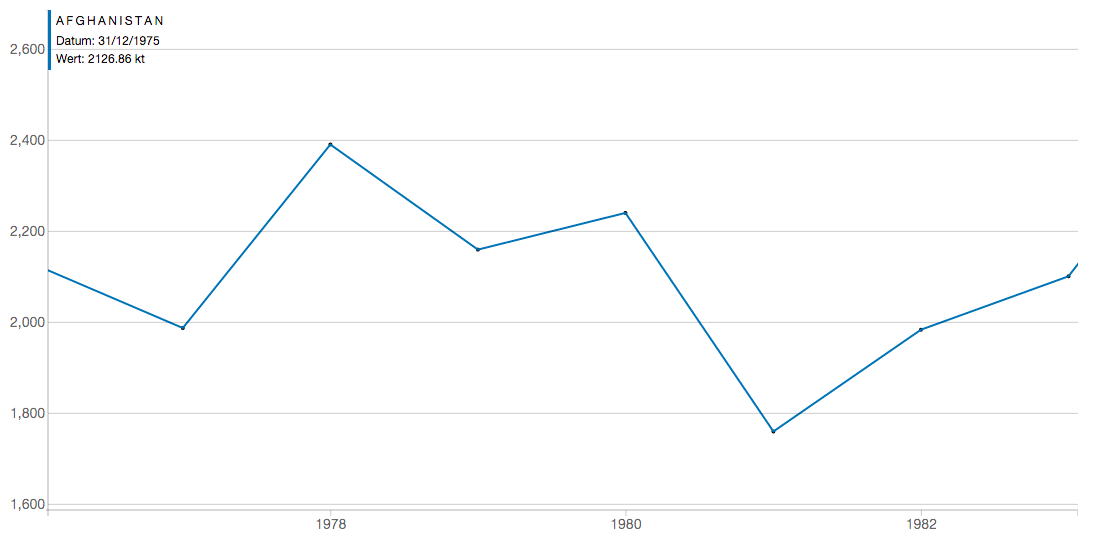
\includegraphics[width=0.80\linewidth]{images/linear}
	\caption[Lineare Interpolation]{Beispiel der linearen Interpolation am Datensatz des CO2-Verbrauchs von Afghanistan.}
	\label{fig:linear}
\end{figure}

Die Interpolation mit Splines, der \textbf{Kubisch Hermitescher Spline} (Abbildung \ref{fig:cardinal}).

\begin{figure}[htbp]
	\centering
	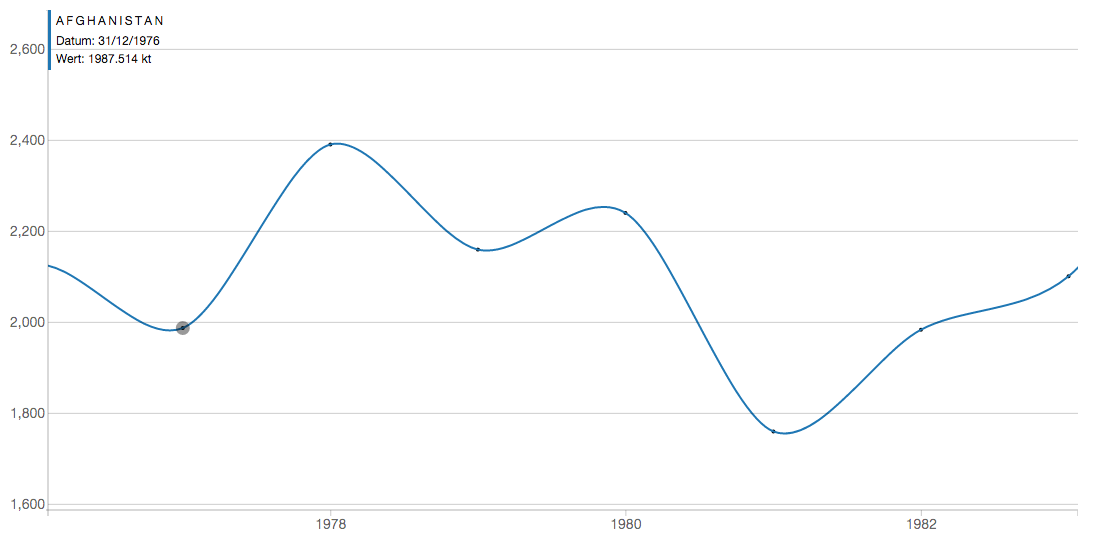
\includegraphics[width=0.80\linewidth]{images/cardinal}
	\caption[Kubischer Hermitescher Spline]{Beispiel des Kubischen Hermetischen Spline am Datensatz des CO2-Verbrauchs von Afghanistan.}
	\label{fig:cardinal}
\end{figure}

\subsection{Linien}
\subsection{Tooltip}
\subsection{Anzeige von mehreren Datensätzen}

\section{3-Dimensionaler Scatterplot}

\subsection{Kamera}
\subsection{Projektion}
\subsection{Orthographische und Perspektivische Kamera}
\subsection{Transition zwischen Projektionen}

\section{n-Dimensionaler Scatterplot}